\documentclass[prl,twocolumn]{revtex4-1}

\usepackage{graphicx}
\usepackage{xcolor}
\usepackage{latexsym,amsmath,amsfonts}
\usepackage{verbatim}
\usepackage{dsfont}
\usepackage{comment}
\usepackage{braket}
\usepackage{mdframed}
\usepackage{booktabs} %tables
\usepackage{ragged2e}
\usepackage{caption}
\usepackage{subcaption}
\usepackage{placeins} % for \FloatBarrier, to force figures in place

\definecolor{linkcolor}{rgb}{0,0,0.65}

\usepackage[
    colorlinks=true,
    pdfstartview=FitV,
    linkcolor=linkcolor,
    citecolor=linkcolor,
    urlcolor=linkcolor,
    hyperindex=true,
    hyperfigures=true
]{hyperref}

\newcommand{\pluseq}{\mathrel{+}=}

\newmdenv[
    topline=false,
    bottomline=false,
    skipabove=\topsep,
    skipbelow=\topsep
]{siderules}


% Ensure numbering is shown
\setcounter{secnumdepth}{2}

% Section: Roman numerals
\renewcommand{\thesection}{\Roman{section}}

% Subsection: Roman.Section + Letter
\renewcommand{\thesubsection}%{\thesection.\Alph{subsection}}
{\Alph{subsection}}

\begin{document}
\title{Markov State Modelling of folding of HP35 domain}
\author{Miriam Zara}
\date{\today}

\begin{abstract}
    In this work, I compare different feature sets and dimensionality reduction methods for the construction of Markov state models (MSMs) of the folding of the HP35 villin headpiece.
\end{abstract}

\maketitle

\section{Introduction}
Biomolecules are dynamical systems that explore complex ensembles of conformations at finite temperature. Molecular dynamics (MD) simulations can provide atomic-level trajectories of these processes, but the resulting data are often too high dimensional to interpret directly. Coarse-grained models are therefore routinely used to facilitate interpretation of simulation data.
In a Markov State Model (MSM), the continuous conformational dynamics is approximated by a Markov chain, which is a stochastic process describing discrete transitions between a finite number of discrete states.  This makes it possible to leverage a well developed mathematical formalism 
to gain insight on both thermodynamics properties (e.g. free energy basins) and kinetic properties (e.g. transition rates and transition pathways) \cite{thebible}.
However, coarse-graining always involves a trade-off between interpretability and information loss. In the case of MSMs, the modelling pipeline includes several steps, such as feature selection, dimensionality reduction, clustering,  and a general optimization criterion is not always available. Different pipelines may result in different models, which raises
the question about which conclusions are physically meaningful and which are to be considered as artefacts.

In this project, I investigate this question through a benchmark study on a simple protein system: the villin headpiece subdomain HP35 Lys24-Nle/Lys29-Nle mutant (Fig.\ref{fig:hp35_structure}). 
HP35 is a short, fast-folding protein that has been extensively used as a model system for protein folding. Long, unbiased, all-atom MD simulations of this system were already available in the early 2010s. In particular, I analyze a 305$\mu$s simulation from \cite{Lindorff-Larsen2011}, 
which contains dozens of folding-unfolding transitions. Because of this extensive sampling, key kinetic quantities such as the folding time and the average transition time have been estimated directly from the trajectory \cite{Piana2012}. 
Previous analysis also reported a free-energy profile in which the system is approximately described by two main states, folded and unfolded, with a low-population intermediate \cite{Piana2012}.
The aim of this project is to test whether different MSM construction pipelines lead to a consistent thermodynamic and structural description of this folding system. 

Operationally, I build four MSMs starting from two internal-coordinate representations, contacts and dihedral angles, and two dimensionality reduction methods, PCA and tICA. I then apply PCCA++ to identify macrostates in each model. The resulting models are compared by asking whether the identified macrostates are consistent across pipelines, whether they 
can be interpreted as metastable states, whether they have a clear structural interpretation in terms of folded, unfolded, and possibly intermediate conformations, and whether their equilibrium populations agree.
Finally, I estimate the folding time and the free-energy gap between macrostates from the MSMs and compare them both across models and with the reference estimates reported in \cite{Piana2012}. 

Overall, this project mostly aims to review the MSM construction pipeline, assess its robustness with respect to modelling choices, and clarify its strengths and limitations for the quantitative analysis of MD simulation data.
%%%%%%%%%%%%%%%%%%%
%
%
%%%%%%%%%%%%%%%%%%%
\section{Methods}
%
\subsection{Dataset assembly}
\begin{figure}[h!]
    \centering
    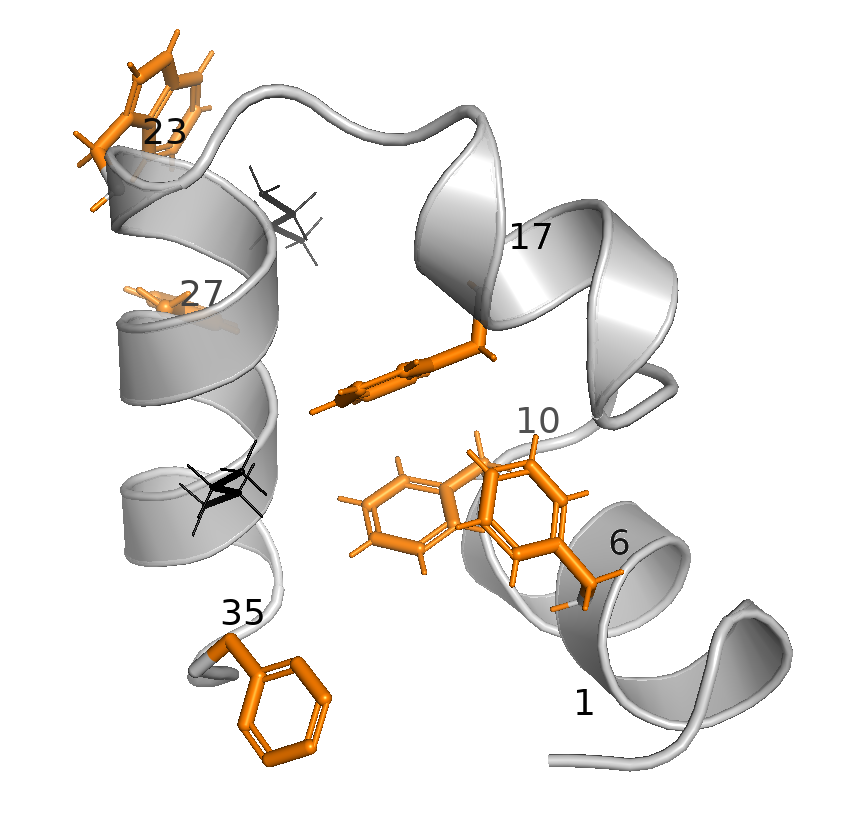
\includegraphics[width=0.5\linewidth]{figures/aromatic_structure.png}
\caption{\small \textbf{Crystal structure of HP35} (PDB: 2F4K \cite{PDB}). The folded structure consists of three $\alpha$-helices, approximately spanning residues 3–10, 14–19, and 22–32, connected by two loops. Aromatic and histidine residues are highlighted in orange: Phe6, Phe10, Phe17, Trp23, His27, and Phe35. Interactions among Phe6, Phe10, and Phe17 contribute to the formation of the hydrophobic core. Visualization was made with PyMOL \cite{pymol}.}
    \label{fig:hp35_structure}
\end{figure}
This work is based on a single $305\,\mu\mathrm{s}$ MD trajectory of the fast-folding Lys24-Nle/Lys29-Nle mutant of the 35-residue villin headpiece subdomain (HP35), simulated at $360\,\mathrm{K}$. 
The original trajectory is reported by Lindorff-Larsen \textit{et al.} \cite{Lindorff-Larsen2011}, while in this project I employ a preprocessed version of that trajectory publicly distributed by Nagel \textit{et al.} \cite{selecting_features}. 
The dataset contains time series of approximately $1.5\times10^6$ samples, with a sampling interval of about $200,\mathrm{ps}$. Authors provide timeseries of two internal-coordinate representations which they selected and filtered specifically for employment in MSM construction, as they describe in detail \cite{selecting_features}.
These are residue-residue contact distances ( \texttt{hp35.mindists2} - $42$ features) and backbone dihedral angles (\texttt{hp35.dihs.shifted} - $62$ features). Authors also provide timeseries of residue-residue distances for a separate set of contacts identified from the crystal structure PDB 2F4K, (\texttt{hp35.crystaldists} - $53$ features).

\subsection{Methods for MSM construction}
All code is written in Python and employs the library Deeptime \cite{deeptime} for MSMs construction, validation and analysis.
The steps involved in MSM construction are, briefly:
\begin{enumerate}
    \setlength{\itemsep}{0.01em}
\item Feature selection,
\item Dimensionality reduction,
\item Clustering of the reduced coordinates into discrete states,
\item Estimation of the transition matrix, selection of lag time and validation of markovianity,
\item Validation of the final model against the data.
\end{enumerate}

In the following I describe briefly the scope and implementation of each step, focusing the most on the two steps that were varied this work, which are 
feature selection and dimensionality reduction. I report more details of the pipeline in the Supplementary Methods \ref{sec:SI_methods}.

MSMs construction at its core necessitates to convert the trajectory frames of the MD simulation into a finite, discrete set of states. 
Ideally, this procedure should preserve the kinetic information of the original continuous dynamics, but with the advantage of being 
much simpler to analyze. The first two steps of the pipeline, feature selection and dimensionality reduction, 
are used to compress the raw MD data in a space that is much lower dimensional, so that a clustering of samples into a finite number of states 
is computationally feasible. Clustering algorithms such as k-means rely on Euclidean distance, so it is important that the reduced coordinates are constructed in such a way that conformations that interconvert rapidly are mapped to nearby points in the reduced space. Otherwise, conformations separated by substantial kinetic barriers may be assigned to the same cluster and the markov property will be violated.
These requirements make the choice of features and dimensionality reduction method a crucial step in the MSM pipeline, and their optimization
is not trivial and has traditionally mostly relied on heuristics. 

I experiment with two different feature sets, which are \texttt{hp35.mindists2} and \texttt{hp35.dihs.shifted} as previously described. As for the dimensionality reduction step, I compared two classical approaches: principal component analysis (PCA) and nd time-lagged independent component analysis (tICA),
for which I provide a detailed derivation in the Supplementary Methods \ref{subsec:SI_dimred}. In short, both methods find linear combinations of the original provided features but with a different optimization objective.
PCA identifies directions of maximal variance in the data, whereas tICA identifies directions of maximal autocorrelation. tICA is explicitly designed to better encode the slow dynamics of the system: while PCA
identifies the degrees of freedom that vary the most, tICA looks for those that vary the most slowly. Therefore, the tICA coordinates are expected to 
encode the slowest degrees of freedom of the system and the notion of euclidean distance in reduced space  defined by tICA is should ideally to be related to a notion of "kinetic distance", with conformations that interconvert rapidly being mapped to nearby points in the reduced space.
tICA is usually found to ouperform PCA in this task, but if this is the case for our system is a question I am going to address. Overall, I build $4$ MSMs, combining the two feature sets and the two dimensionality reduction methods: tica-distances, tica-dihedrals, pca-distances and pca-dihedrals.
\vspace{0.5em}\newline
\textit{Clustering:}
The reduced coordinates were clustered using k-means with $100$, $200$, and $500$ clusters.
Cluster centres were initialized uniformly and the algorithm was run for a maximum of $100$ iterations. Transition matrices were estimated using a maximum-likelihood 
MSM estimator at lag times $\tau$ ranging from $10$ to $1000$ frames ($\sim 2-200\,ns$). The counting scheme used was the "sliding window" scheme, which counts transitions at every time step, as opposed to the "discrete" scheme, which counts transitions only at multiples of $\tau$ \cite[Chap. 4.1]{thebible}.
Detailed balance was enforced during the estimation of the transition matrix and the largest connected component was taken as the state space of the MSM.
The range of lagtimes investigated was chosen to remain substantially shorter than the characteristic folding timescale ($\sim 1-3 \,\mu s$), ensuring that the process of interest
remained temporally resolved.
\newline \textit{Lagtime choice:}
Estimation of the transition matrix requires specification of the lag time $\tau$ ($= 1, 2, 3\cdots$ in number of frames) at which to count transitions between states. Choice of lag time is done through the
timescale convergence test. Briefly (see \ref{suppsec:markov_theory}), the transition matrix $T(\tau)$  is estimated at different lag times and its eigenvalues are used to compute the implied timescales $t_i(\tau)$, which are then plotted as a function of $\tau$. 
If the Markovian assumption is valid, the implied timescales should be approximately constant for sufficiently large $\tau$. The lag time is then selected as the minimum value in the region of convergence, as this choice minimizes the loss of temporal resolution while ensuring that the process of interest is approximately Markovian\cite[Ch. 4.7]{thebible}.
\newline \textit{MSM validation:} to validate the model against the original trajectory, I compare the autocorrelation function of the root mean square deviation (RMSD) to the crystal structure computed from the trajectory (\texttt{hp35.crystaldist}) and predicted by the MSMs (see \ref{suppsec:markov_theory}).
%
%
%
\subsection{Methods for MSM analysis}
The spectral analysis of the transition matrix provides a natural framework to characterize the dynamical processes captured by the MSM in terms of eigenvalues and eigenvectors. Eigenvalues are related to the relaxation timescales of the system, while eigenvectors encode the states participating in each relaxation process (see \ref{suppsec:markov_theory}).
PCCA++ \cite[Ch. 2.5.1 and 2.5.2]{thebible} is a systematic algorithm to identify metastable states in the MSM by partitioning the microstates based on the signs of the eigenvector components associated with the slowest relaxation processes. \textcolor{blue}{Add other things you use}
%%%%%%%%%%%%%%%%%%%%%%%%%%%%%%%%%%%%%%%%%%%%%%%%%%%%%%%%%%%%%%%%%%%%%%%%%%%%%%%%%%%%%%%%%%%%%%%%%
%
%
%
%
%
%
%%%%%%%%%%%%%%%%%%%%%%%%%%%%%%%%%%%%%%%%%%%%%%%%%%%%%%%%%%%%%%%%%%%%%%%%%%%%%%%%%%%%%%%%%%%%%%%%%
\section{Results}
\subsection{Construction of the MSMs} 
\begin{figure*}[ht]
    \centering
    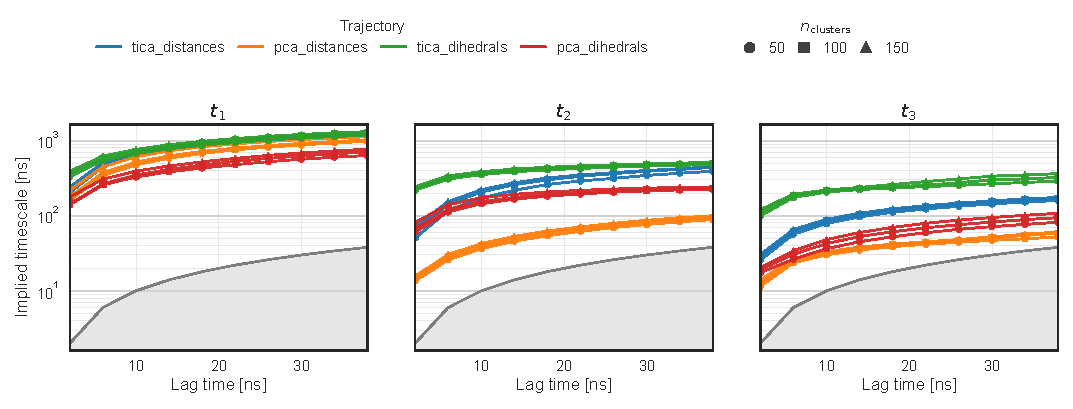
\includegraphics[width=0.7\linewidth]{figures/implied_timescales_report.pdf}
    \caption{\footnotesize Results of the MSM construction pipeline. \textbf{Middle left.}
     First three implied timescales as a function of the MSM lagtime. Colors denote the four combinations of feature set and dimensionality reduction method, while marker styles indicate the number of microstates used in the state-space discretization. 
        The shaded region corresponds to $t_i \leq \tau$, where $t_i$ is the implied timescale and $\tau$ the MSM lagtime. Timescales falling within this region are not resolved by the model, 
        as the associated relaxation process occurs on a timescale shorter than a single Markov-chain transition step.}
    \label{fig:msm_results}
\end{figure*}
Both PCA and tICA require selecting the number of retained components, while tICA additionally requires specifying a lag time. To guide this choice, I use this heuristic criteria:
the reduced coordinates were evaluated through i) their free-energy profiles and ii) projected time series. The rationale behind this analysis is that coordinates relevant to the folding process should separate distinct metastable regions
and therefore display multimodal free-energy profiles. Furthermore, if a coordinate captures transitions between metastable states, its time series should exhibit relatively long-lived plateaus separated by rapid transitions.
For tICA, lag times between $100$ and $1000$ frames (approximately $20-200$ ns) were considered, since HP$35$ is known to fold a microsecond timescale, 
the autocorrelation  be inspected at times shorter than this timescale. The tICA projections obtained using lag times between $100$ and $1000$ frames ($20-200$ ns) looked qualitatively similar. I selected a tICA lag time of $1000$ frames ($200$ ns).
Overall, dihedral-angle features appear to retain a richer kinetic structure than pairwise-distance features. In the tICA representation, more than seven dihedral components displayed bimodal or multi-modal free-energy profiles and transition-like time series, whereas distance-based features exhibited such behaviour 
only for approximately the first three components.  For PCA, the same visual analysis suggests generally worse performance compared to tICA, with fewer components displaying transition-like timeseries and bimodal free energy profiles.
I use the following number of components: $7$ for tica-dihedrals, $5$ for the others. From a projection onto the first $2D$ components made just for visualization, it appears that all four reduced representations are able to separate the folded and unfolded configurations, at varying degree (see Fig.\ref{fig:msm_results}).
The implied timescale test indicates approximate convergence of the slowest dynamical processesfor MSM lagtimes in the range of $20$-$50,\mathrm{ns}$ as shown in Fig.\ref{fig:msm_results}.
The estimated timescales depend much more strongly on the choice of feature set and dimensionality reduction method than on the number of microstates
used in the discretization (here, tried as $100, 200$ and $500$). For all four feature-reduction pipelines considered, the slowest implied timescale is in reasonable agreement ($\simeq 1-2\, \mu s$), 
whereas larger discrepancies are observed for the higher-order timescales. The pipeline dihedrals-tICA consistenltly yelds the largest timescales, followed by distances-tICA, indicating more accurate approximation
of the underlying continuous dynamics. Validation was performed as described in Methods comparing the autocorrelation function of the RMSD to the crystal structure computed from the trajectory and predicted by the MSMs (see Fig.\ref{fig:autocorrelation}).
The dihedrals-tICA, distance-tICA and distances-PCA pipeline yield similar results, while the pca-dihedrals performs substantially {\color{orange} ? - need uncertainties} worse.

%%%%%%%%%%%%%%%%%%%%%%%%%%%%%%%%%%%%%%%%%%%%%%%%%%%%%%%%%%%%%%%%%%%%%%%%%%%%%%%%%%%%%%%%%%%%%%%%%%
%
%%%%%%%%%%%%%%%%%%%%%%%%%%%%%%%%%%%%%%%%%%%%%%%%%%%%%%%%%%%%%%%%%%%%%%%%%%%%%%%%%%%%%%%%%%%%%%%%%\
\subsection{Analysis of the MSMs} 
\begin{figure}[h!]
    \centering
    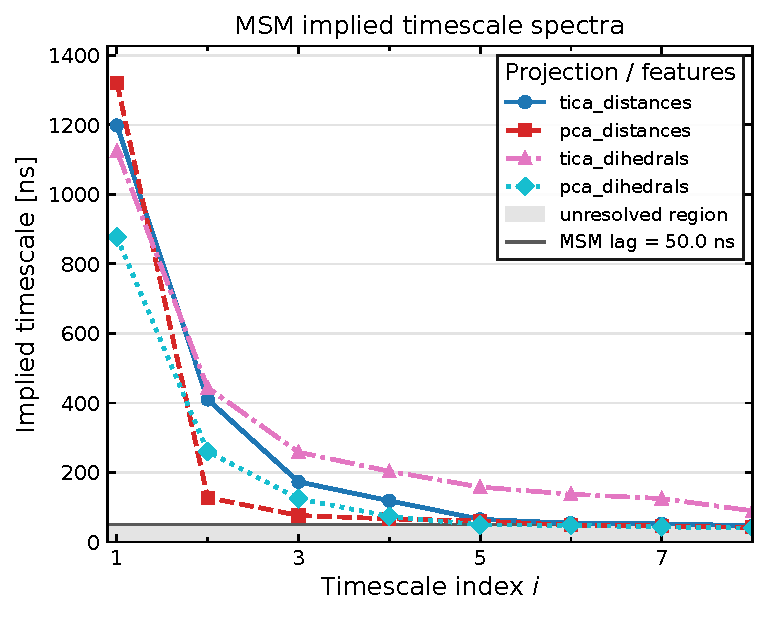
\includegraphics[width = 0.7\linewidth]{figures/msm_timescale_spectra_report.pdf}
    \caption{The timescales spectra for the four markov models}
    \label{fig:timescales_spectra}
\end{figure}

The timescale spectra of the four models Fig. \ref{fig:timescales_spectra} highlight some differences between the four models. The two PCA-based models have a clear gap between the first and second timescale, suggesting that a two-state model is a good approximation of the dynamics. Instead, the two
tICA-based models display the largest gap between the second and the third timescale, suggesting that a three-state model would be a better approximation. It is possible that the tICA models are able to resolve one of the two basins in more details, while the PCA models cannot, but this hypotesis needs to be checked. 
\subsubsection{Two-state PCCA++}
As a starting point, I will consider a two-state model for all four MSMs, and I will check whether the two macrostates identified by PCCA++ are consistent across models and interpretable.
I expect that the slowest timescale corresponds to the folding-unfolding process, and therefore that the two macrostates correspond to the folded and unfolded basins. A first qualitative
support of this hypotesis is found by inspecting the sign pattern of the first right eigenvector and comparing it with a structural descriptor of folding, like the fraction of native contacts $Q$ (see Supp. Figure \ref{suppfig:first_right_eigenvector}).

I apply PCCA++ with $2$ macrostates to all four models, and I compute the fuzzy membership probabilities of  i) microstates and ii) single trajectory frames.

I check the distribution of the fuzzy membership probabilities of frames across models (see Fig. \ref{suppfig:fuzzy_memberships_models}). This shows a high model agreement in the assignation of frames to macrostates.
I also quantify model agreement by computing the overlap between the "core" subsets. I identify as "cores" the sets of frames where the probability of assignation is $p<0.4$ for macrostate $S0$ and $p>0.6$ for macrostate $S1$. I compute the Jaccard index as a simple measure of overlap. Results 
show very high agreement among the models on the definition of macrostate $S1$, while high but not perfect agreement in the definition of $S0$, which indicates that each model places the boundary between the two macrostates in a slightly different manner (Supp. Table \ref{supptab:jaccard_core_overlap}).
Next I compute the populations of the two macrostates, considering fuzzy assignments:
$$
P(S_i) = \frac{1}{N} \sum_{j=1}^{N} P(x_j \in S_i) \cdot \pi_j
$$
where $N$ is the number of microstates, $P(x_j \in S_i)$ is the fuzzy membership probability of microstate $j$ to macrostate $i$, and $\pi_j$ is the stationary probability of microstate $j$.
The results are reported in Table \ref{tab:pcca_two_state_populations} together with the estimated free energy difference. 
Estimated populations are in reasonable agreement between the models, and the estimated free energy differences are reasonably consistent with the reference value of $-0.6\pm 0.2$ kcal/mol reported in \textit{Piana et. al.} \cite{Piana2012}. 

\begin{table}[h!]
\caption{Coarse-grained stationary populations of the two PCCA macrostates for each MSM at the common two-state resolution. Relative free energies were computed as $\Delta G_{1-0} = -k_B T \ln[P(S_1)/P(S_0)]$ with $T=360$ K.}
\label{tab:pcca_two_state_populations}
\begin{tabular}{lccc}
\hline
Model & $P(S_0)$ & $P(S_1)$ & $\Delta G_{1-0}$ (kcal mol$^{-1}$) \\
\hline
tica\_distances & 0.215 & 0.785 & -0.928 \\
pca\_distances & 0.299 & 0.701 & -0.609 \\
tica\_dihedrals & 0.223 & 0.777 & -0.891 \\
pca\_dihedrals & 0.332 & 0.668 & -0.500 \\
\hline
\end{tabular}
\end{table}

To assess with certain that macrostate S$1$ is identificable with the folded basin, I proceed to structural caracterization. To avoid biasing the analysis by boundary-like frames, I select only the frames that are assigned to the native basin by all four models. These are $67\%$ of total simulation frames.
Possibly the easiest caracterization of the native basin is in terms of contacts. I compute statistics  of distances for all contacts in the crystal structure (\texttt{hp.crystaldist}), and I compare the distributions in the native basin with those in the rest of the trajectory.
I define a simple, heuristic score to quantify the importance of each contact for discrimination of the native basin. The score is based on the shift in the median and the interquartile range (IQR) of the distance distributions in the native basin and in the rest of the trajectory.
$$
d^{\mathrm{robust}}_{ij}
=
\frac{
\mathrm{median}(r_{ij}^{\mathrm{other}})
-
\mathrm{median}(r_{ij}^{\mathrm{folded}})
}{
\mathrm{IQR}_{\mathrm{pooled}}
}
$$

This expresses that a contact is important for differentiating the basin if its distance distribution is substantially shifted toward shorter distances in the folded basin and substantially more narrow in the folded basin.
The $10$ most important contacts according to this score are reported in Supp. Table \ref{tab:top10_folded_contacts}. A visual representation of the most important contacts is shown in Fig. \ref{fig:contact_map_folded_vs_other}, together with the visualization of a representative set of structures.
It is evident that the most important contacts for discrimination of the folded basin are those that form the hydrophobic core, in particular a set of contacts in the neighbourhood of Phe6 and Phe10. Instead,
the contacts defining the three helices are the least important, which is consistent with the fact that the helices are formed in both folded and unfolded configurations, while the hydrophobic core is only formed in the folded basin. 
\begin{figure}[h!]
    \centering
    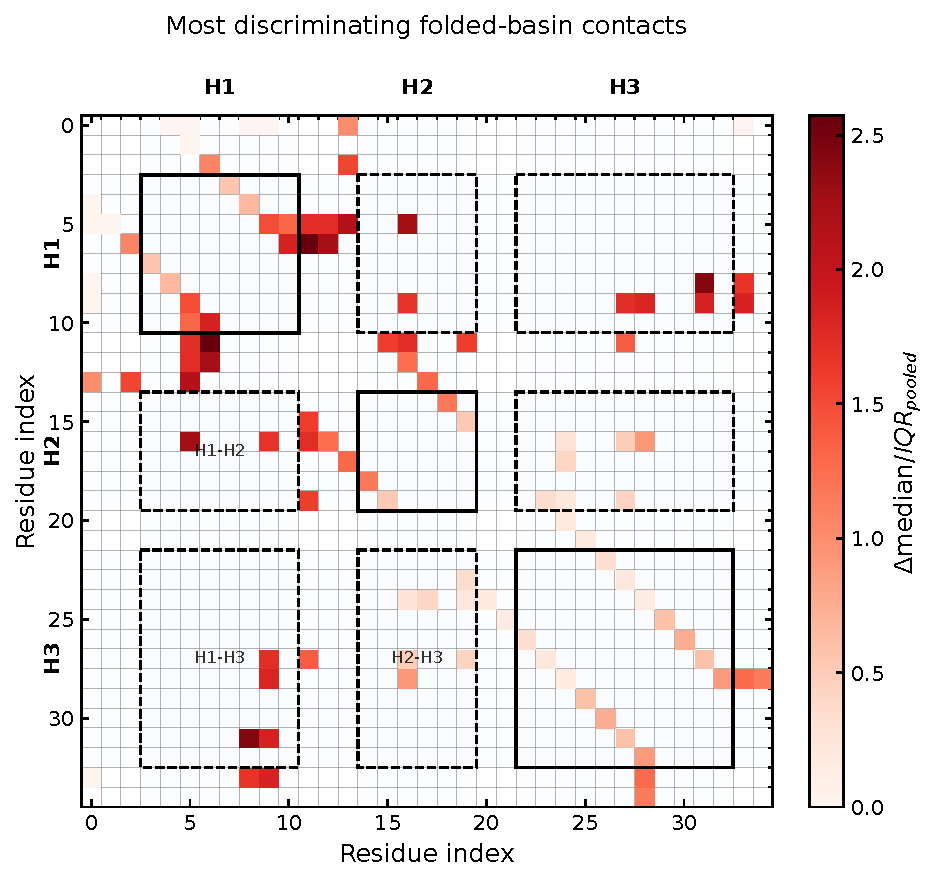
\includegraphics[width = 0.8\linewidth]{figures/folded_basin_contact_map_report.pdf}
    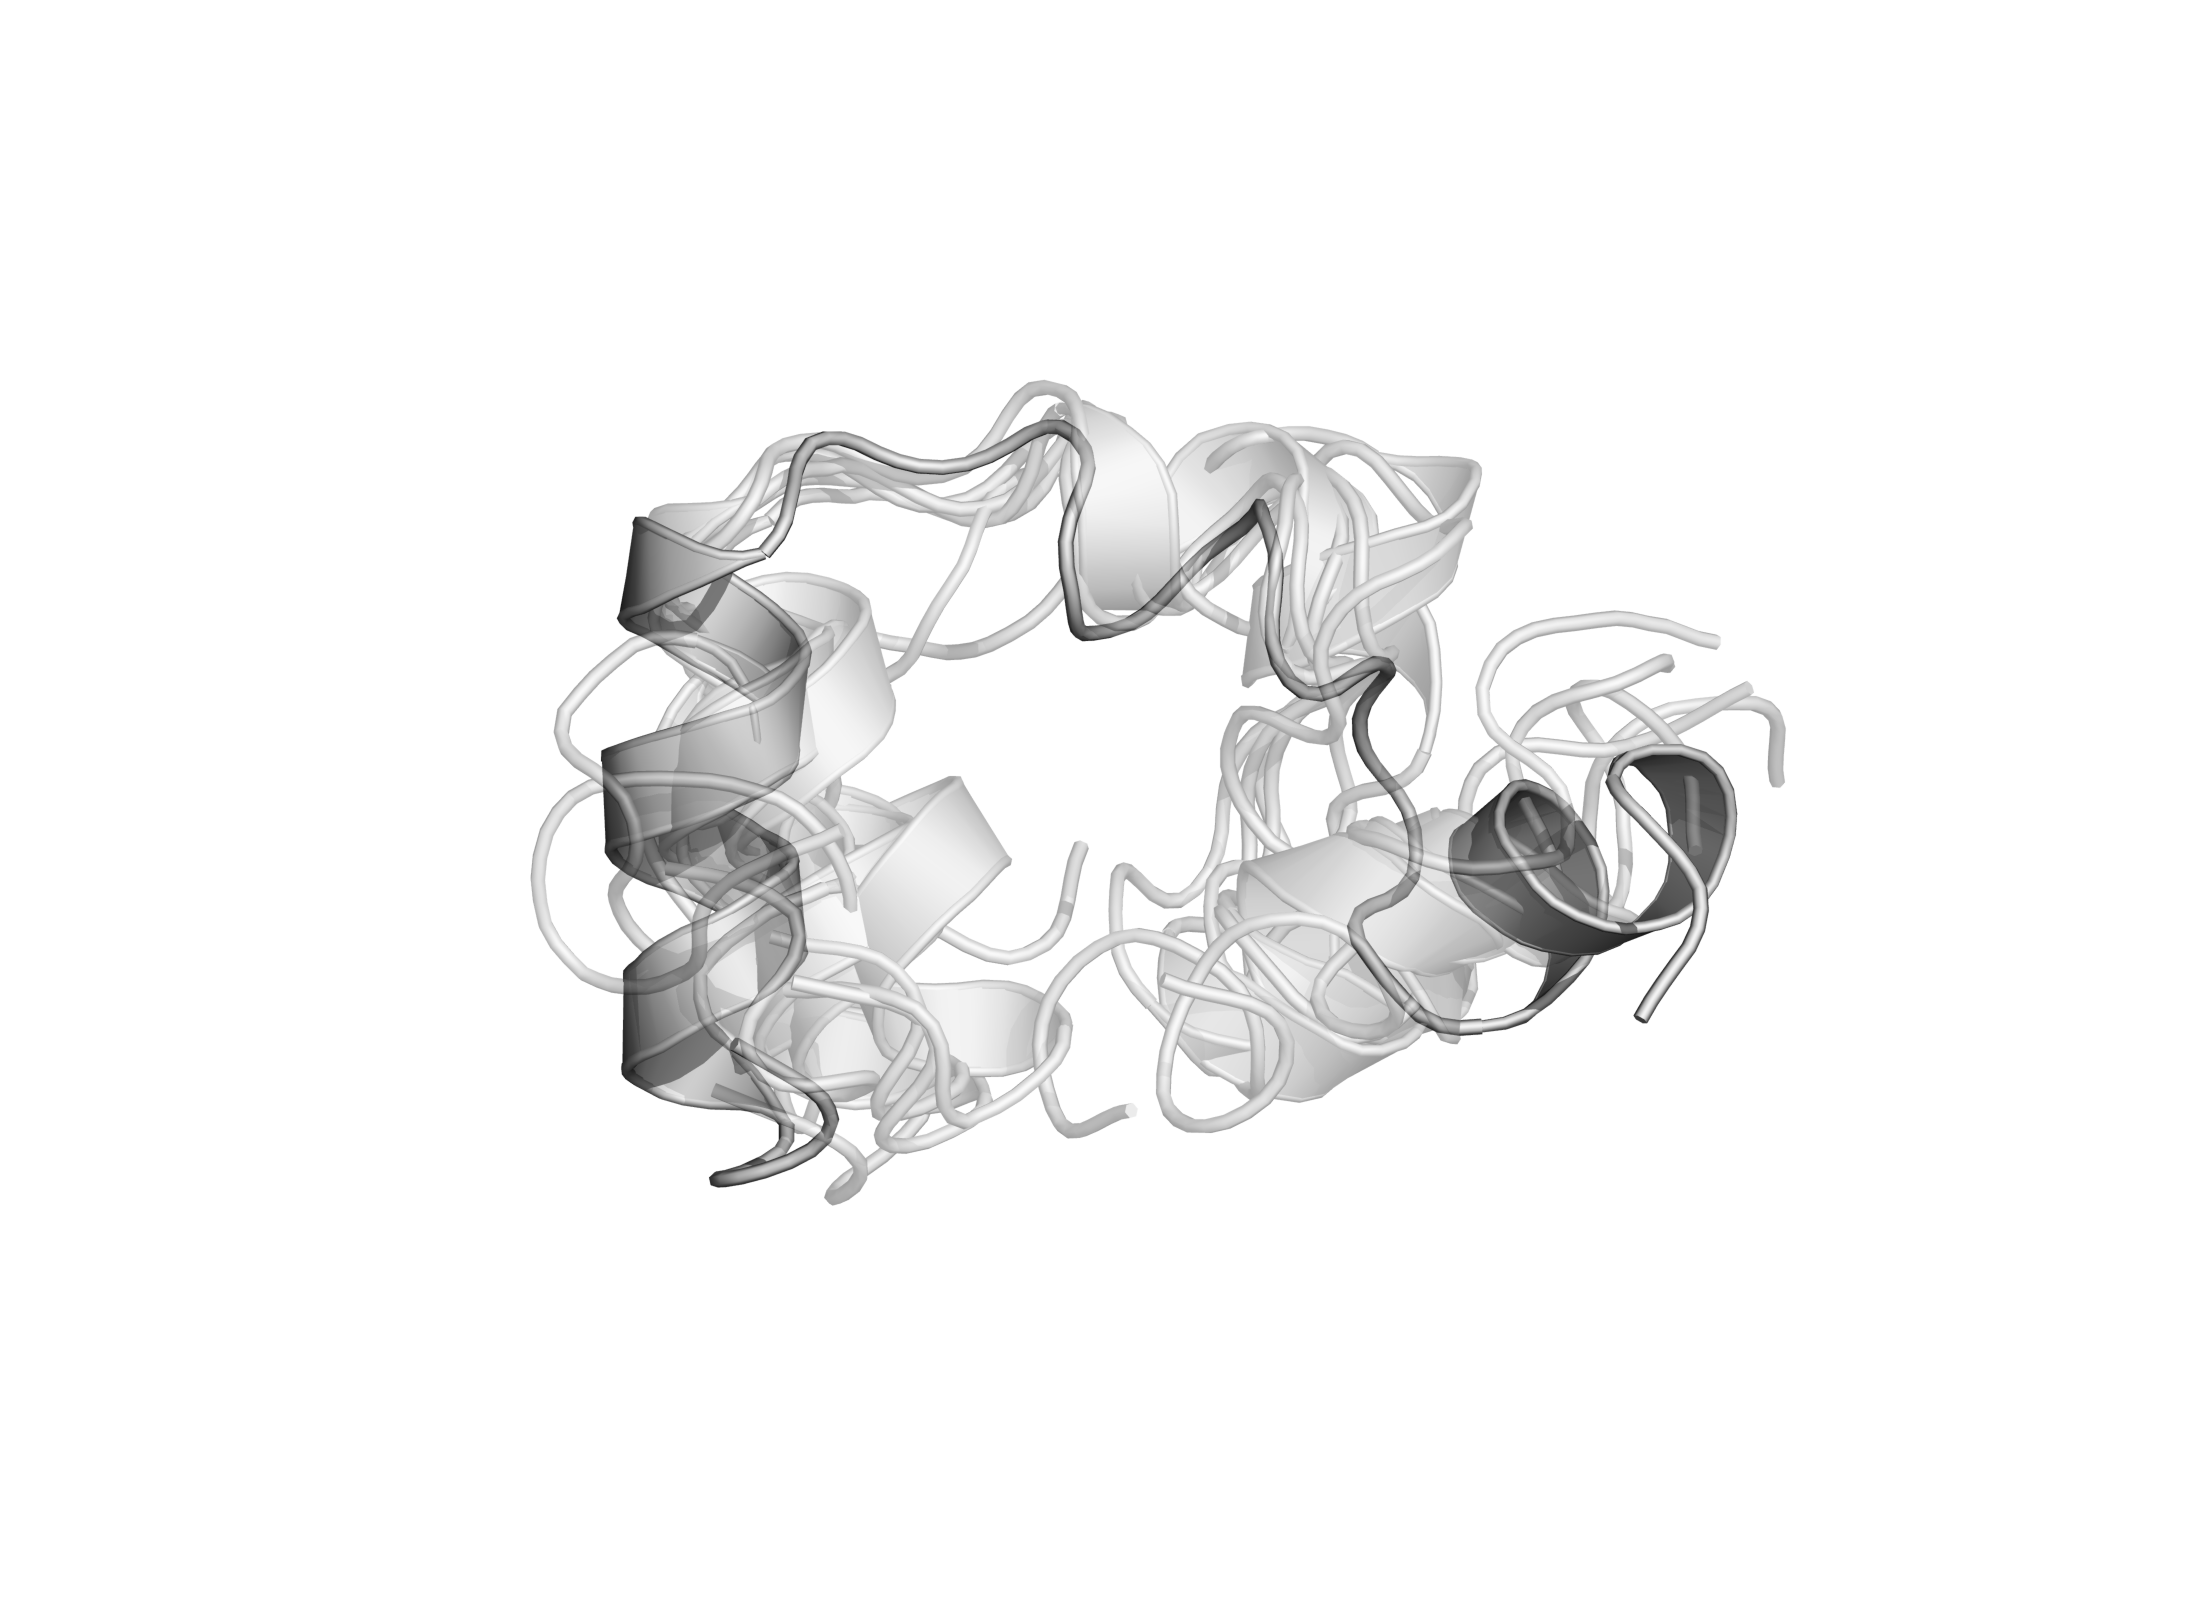
\includegraphics[width = \linewidth]{figures/native_basin_ensemble_overlay_ray.png}
    \caption{Caracterization of consensus frames. Top: contact map of the crystal structure (PDB 2F4K) where the color scale indicates the importance of each contact for discrimination of the folded basin as explained in the text.
    Bottom: overlay of a random sample of $5$ structures from the consensus folded basin. Visualization was made with PyMOL \cite{pymol}.}
    \label{fig:contact_map_folded_vs_other}
\end{figure}

To conclude this analysis I will provide an indicative estimate the folding time as the average waiting time in the folded basin. This is only indicative, as for an accurate estimate of the folding time one should consider the full microstate model and use transition path theory, which is not done here.
A first rough estimate can be obtained from the transition matrix of the coarse-grained PCCA++ model:

$$
\langle t_{\mathrm{folded}} \rangle = \frac{\tau}{T_{01}},
$$

where $T_{01}$ is the transition probability from macrostate $S_0$ to macrostate $S_1$ and $\tau$ is the lagtime of the MSM. A second rough estimate can be obtained from the trajectory by computing the average waiting time in the folded basin, which is defined as the average time between two consecutive transitions from the unfolded to the folded basin. The results are reported in Table \ref{tab:folding_times}. 
The two estimates are in reasonable agreement, and they are also consistent with the reference value of $3.2\pm 0.6\,\mu s$ reported in \cite{Piana2012}.
%%%%%%%%%%%%%%%%%%%%%%%%%%%%%%%%%%%%%%%%%%%%%%%%%%%%%%%%%%%%%%%%%%%%%%%%%%%%%%%%%%%%%%%%%%%%%%%%%
%
%
%
%
%
%
%
%

%
%%%%%%%%%%%%%%%%%%%%%%%%%%%%%%%%%%%%%%%%%%%%%%%%%%%%%%%%%%%%%%%%%%%%%%%%%%%%%%%%%%%%%%%%%%%%%%%%%

\FloatBarrier

\section{Discussion}
{\color{blue}
Here you try to put your results into a broader context and present your scientific view/model based on that. This is a continuous text, broken into paragraphs. 
In case you have two distinct 'huge' conclusions, you may generate separate sections (max 2). Chapter 4 should be organised as follows:
\begin{itemize}
\item You may phrase your biological question again.
\item Briefly summarise the results (max one paragraph). You do not repeat the words you used earlier, make it concise. Make it evident how your results ansIr the question you have asked.
\item Compare your results with something in the literature (use PubMed, or literature indicated in UniProt, PDB or any datasets I learnt about). 1-2 articles enough. The point is that you
\item show how your results relate to previous ones. Different scenarios: 'support', 'in contrast', 'in addition', 'gives insights into'.
\item If possible, present a model. This can be a molecular 'mechanism', 'scenario', 'reason'. For example: 'A and B belong to the same family'; 'mutation XD likely changes the interaction in liver'; 'in disease T I have less phosphorylation sites or the level of phosphorylation decreased'; 'in this experiment, there is a problem with degradation of protein P. ' etc.
\item The model can be presented as: 'propose', 'suggest', 'indicate','hypothesize', or even 'support' or 'demonstrate'. If possible try to present a cartoon figure or scheme.
\end{itemize}
}
%%%%%%%%%%%%%%%%%%%%%%%%%%%%%%%%%%%%%%%%%%%%%%%%%%%%%%%%%%%%%%%%%%%%%%%%%%%%%%%%%%%%%%%%%%%%%%%%%
%
%
%
%%%%%%%%%%%%%%%%%%%%%%%%%%%%%%%%%%%%%%%%%%%%%%%%%%%%%%%%%%%%%%%%%%%%%%%%%%%%%%%%%%%%%%%%%%%%%%%%%
\section{Conclusions}
{ \color{blue}
One paragraph, emphasizing the main finding and formulate a message for the future (perspective), how to continue from here, what kind of further studies are needed. You may have Conclusion as chapter 5.
}
%%%%%%%%%%%%%%%%%%%%%%%%%%%%%%%%%%%%%%%%%%%%%%%%%%%%%%%%%%%%%%%%%%%%%%%%%%%%%%%%%%%%%%%%%%%%%%%%%
%
%
%
%%%%%%%%%%%%%%%%%%%%%%%%%%%%%%%%%%%%%%%%%%%%%%%%%%%%%%%%%%%%%%%%%%%%%%%%%%%%%%%%%%%%%%%%%%%%%%%%%
\section{References}
{ \color{blue}
The text should contain references, to previous results, data, methods, softwares, etc.. Format is unrestricted, but you should use these refs in the text, and list them at the end. I expect ca 15-20 refs listed.
}
\newline \noindent \textbf{Data availability statement:} Preprocessed trajectories of the HP35 villin headpiece are kindly made available by Nagel et al. and downloadeable at their GitHub repository \url{https://github.com/moldyn/HP35-DESRES}.
All code necessary to replicate the analysis shoId in this work is available on GitHub at \url{https://github.com/miriamzara/MSM}.

\begin{thebibliography}{99}
\setlength{\itemsep}{3pt}  % adjust to taste

% --------------------------------------------------------
% -------- HP35 specific references ----------------------

\bibitem{Lindorff-Larsen2011}
    K. Lindorff-Larsen, S. Piana, R.O. Dror and D.E. Shaw,  
    \textit{How fast-folding proteins fold}, 
    Science 334 (6055) 517-520 (2011), 
    DOI: 10.1126/science.1208351.


\bibitem{Piana2012}
    S. Piana, K. Lindorff-Larsen and D.E. Shaw,  
    \textit{Protein folding kinetics and thermodynamics from atomistic simulation}, 
    Proc. Natl. Acad. Sci. U.S.A. 109 (44) 17845-17850 (2012), 
    DOI: 10.1073/pnas.1201811109.

\bibitem{PDB}
    J. Kubelka, T.K. Chiu, D.R. Davies et al.,
    \textit{Sub-microsecond protein folding},
    J. Mol. Biol. 2006, 359, 546-553.
    DOI: 10.1016/j.jmb.2006.03.034.


\bibitem{selecting_features}
    D. Nagel, S. Sartore, and G. Stock,
    \textit{Selecting Features for Markov Modeling: A Case Study on HP35},
    Journal of Chemical Theory and Computation 2023 19 (11), 3391-3405
    DOI:  10.1021/acs.jctc.3c00240.

\bibitem{towards_a_benchmark}
    D. Nagel, S. Sartore, and G. Stock,
    \textit{Toward a Benchmark for Markov State Models: The Folding of HP35},
    The Journal of Physical Chemistry Letters 2023 14 (31), 6956-6967
    DOI:  10.1021/acs.jpclett.3c01561 .
    
%\bibitem{jain_stock_2014}
%    A. Jain and G. Stock,
%    \textit{Hierarchical Folding Free Energy Landscape of HP35 Revealed by Most Probable Path Clustering}
%    J. Phys. Chem. B, 118, 28, 7750-7760 (2014).
%    DOI: 10.1021/jp410398a.


\bibitem{thebible}
    G.R. Bowman, V.S. Pande and F. Noé,
    \textit{An Introduction to Markov State Models and Their Application to Long Timescale Molecular Simulation}
    Advances in Experimental Medicine and Biology, Springer Dordrecht (2013)
    DOI:  10.1007/978-94-007-7606-7.


\bibitem{deeptime}
   M. Hoffmann, M.K. Scherer, T. Hempel et al.,
  \textit{Deeptime: a Python library for machine learning dynamical models from time series data},
  Machine Learning: Science and Technology, 2021, IOP Publishing.
DOI: 10.1088/2632-2153/ac3de0.


%\bibitem{vampnets}
%  A. Mardt, L. Pasquali, H. Wu and F. No\'e,
%  \textit{VAMPnets for deep learning of molecular kinetics},
%  Nature Communications 9(1):1-11, 2018. 

%\bibitem{time_lagged_autoencoders}
%    C. Ihmeyer and F. No\'e. 
%    \textit{Time-lagged autoencoders: deep learning of slow collective variables for molecular kinetics}. 
%    J. Chem. Phys., 148(24):241703, 2018. 
%    DOI: 10.1063/1.5011399.

%\bibitem{vamp_2013}
%    F. No\'e and F. Nüske,
%    \textit{A variational approach to modeling slow processes in stochastic dynamical systems},
%    Multiscale Modeling \& Simulation 11(2):635-655, 2013.
%    DOI: 10.1137/12089574X.

%\bibitem{vamp_2020}
%    H. Wu and F. Noé,
%    \textit{Variational approach for learning markov processes from time series data},
%    Journal of Nonlinear Science 30(1):23-66, 2020.
%    DOI: 10.1007/s00332-019-09576-8.

%\bibitem{Sittel2017}
%    F. Sittel, T. Filk and G. Stock,
%    \textit{Principal component analysis on a torus: Theory and application to protein dynamics}
%    J Chem Phys. 147(24):244101, 2017.  
%    DOI: 10.1063/1.4998259.


%\bibitem{MoSAIC}
%   G. Diez, D. Nagel and G. Stock,
%   \textit{Correlation-based feature selection to identify functional dynamics in proteins.} 
%   J. Chem. Theory Comput. 2022, 18, 5079-5088.
%   DOI: 10.1021/acs.jctc.2c00337.

\bibitem{my_tica_ref}
    C.R. Schwantes and V.S. Pande,
    \textit{Improvements in Markov State Model Construction Reveal Many Non-Native Interactions in the Folding of NTL9}
    J. Chem. Theory Comput. 2013, 9, 4, 2000-2009
    DOI: 10.1021/ct300878a.


\bibitem{pymol}
    \textit{PyMOL}
    The PyMOL Molecular Graphics System, Version 3.0 Schrödinger, LLC.
\end{thebibliography}
%%%%%%%%%%%%%%%%%%%%%%%%%%%%%%%%%%%%%%%%%%%%%%%%%%%%%%%%%%%%%%%%%%%%%%%%%%%%%%%%%%%%%%%%%%%%%%%%%
%
%
%
%%%%%%%%%%%%%%%%%%%%%%%%%%%%%%%%%%%%%%%%%%%%%%%%%%%%%%%%%%%%%%%%%%%%%%%%%%%%%%%%%%%%%%%%%%%%%%%%%

\appendix

%%%%%%%%%%%%%%%%%%%%%%%%%%%%%%%%%%%%%%%%%%%%%%%%%%%%%%%%%%%%%%%%%%%%%%%%%%%%%%%%%%%%%%%%%%%%%%%%%
%
%
%
%%%%%%%%%%%%%%%%%%%%%%%%%%%%%%%%%%%%%%%%%%%%%%%%%%%%%%%%%%%%%%%%%%%%%%%%%%%%%%%%%%%%%%%%%%%%%%%%%
\clearpage
\onecolumngrid
\section{Supplementary Figures}
\setcounter{figure}{0}
\renewcommand{\thefigure}{SF\arabic{figure}}



% --------------- Dim red time series and free energy profiles
\begin{figure}[h!]
    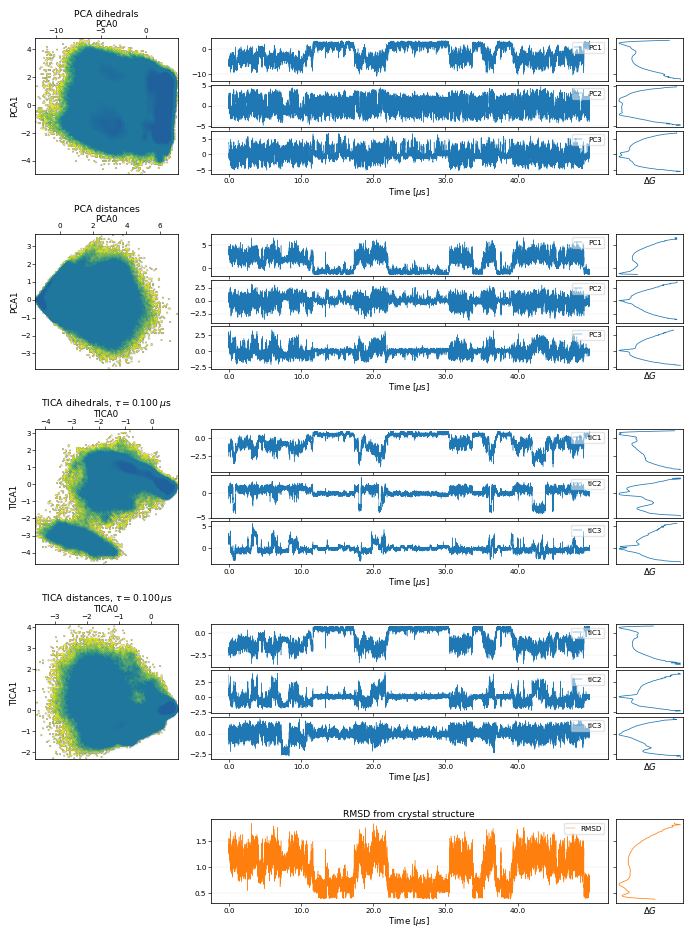
\includegraphics[width=0.7\linewidth]{figures/dimred_figure.png}
\caption{\small
Comparison of the compressed trajectory representations obtained from the four feature--dimensionality-reduction pipelines. 
Rows correspond to PCA dihedrals, PCA contact distances, TICA dihedrals, and TICA contact distances. 
The left column shows the projection onto the first two reduced coordinates. 
The right block shows, for each pipeline, the time series of the first three reduced coordinates over the first $40\,\mu\mathrm{s}$, together with the corresponding one-dimensional free-energy profiles computed from the full trajectory. 
The bottom row reports the RMSD from the crystal structure and its one-dimensional free-energy profile as a reference folding coordinate. 
The PCA projections show mostly unimodal one-dimensional free-energy profiles and less pronounced residence-and-jump behavior with respect to the tICA representations. 
}
    \label{suppfig:dimred_figure}
\end{figure}


% --------------- MSM connectivity and active population as a function of lag time
\begin{figure}[h!]
    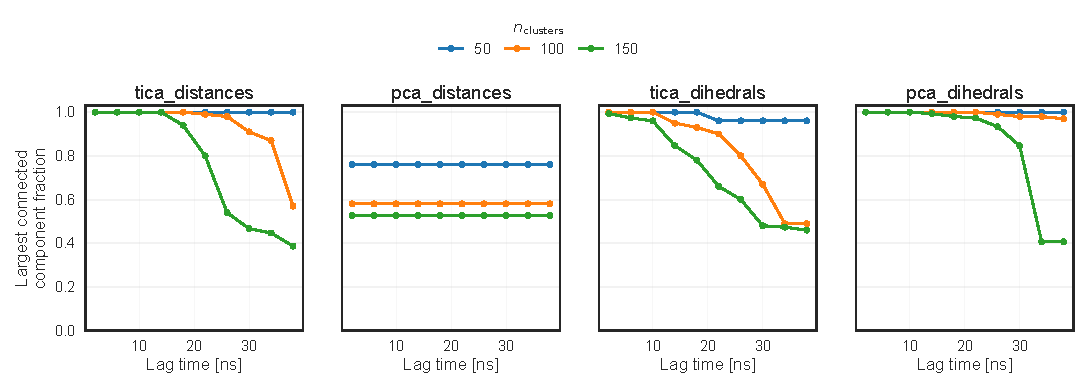
\includegraphics[width=0.7\linewidth]{figures/largest_connected_component_vs_lag.pdf}
    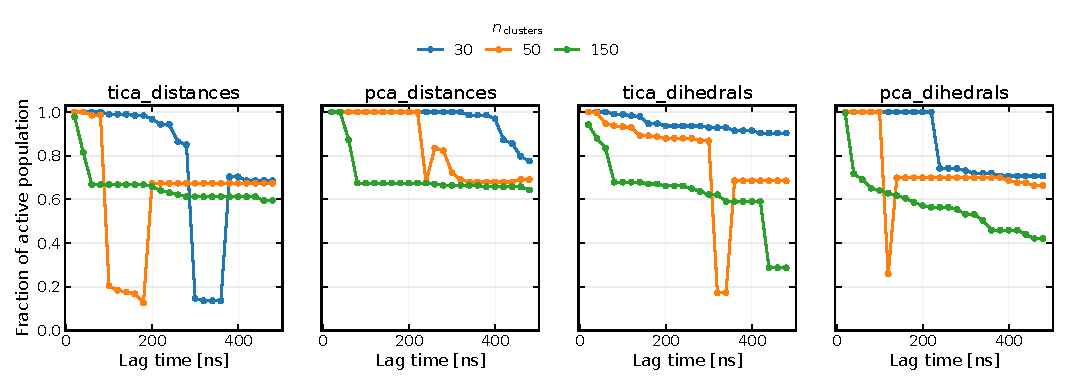
\includegraphics[width=0.7\linewidth]{figures/active_population_vs_lag.pdf}
    \caption{\small \textbf{MSM connectivity and active population as a function of lag time.}
    Top panel: fraction of microstates in the largest connected component of the MSM as a function of lag time. 
    Bottom panel: fraction of the total equilibrium population contained in the largest connected component of the MSM as a function of lag time}
    \label{suppfig:largest_connected_component_vs_lag}
\end{figure}



% ------------- First eigenvector of all models -------------------------
\begin{figure}[!t]
    \centering
    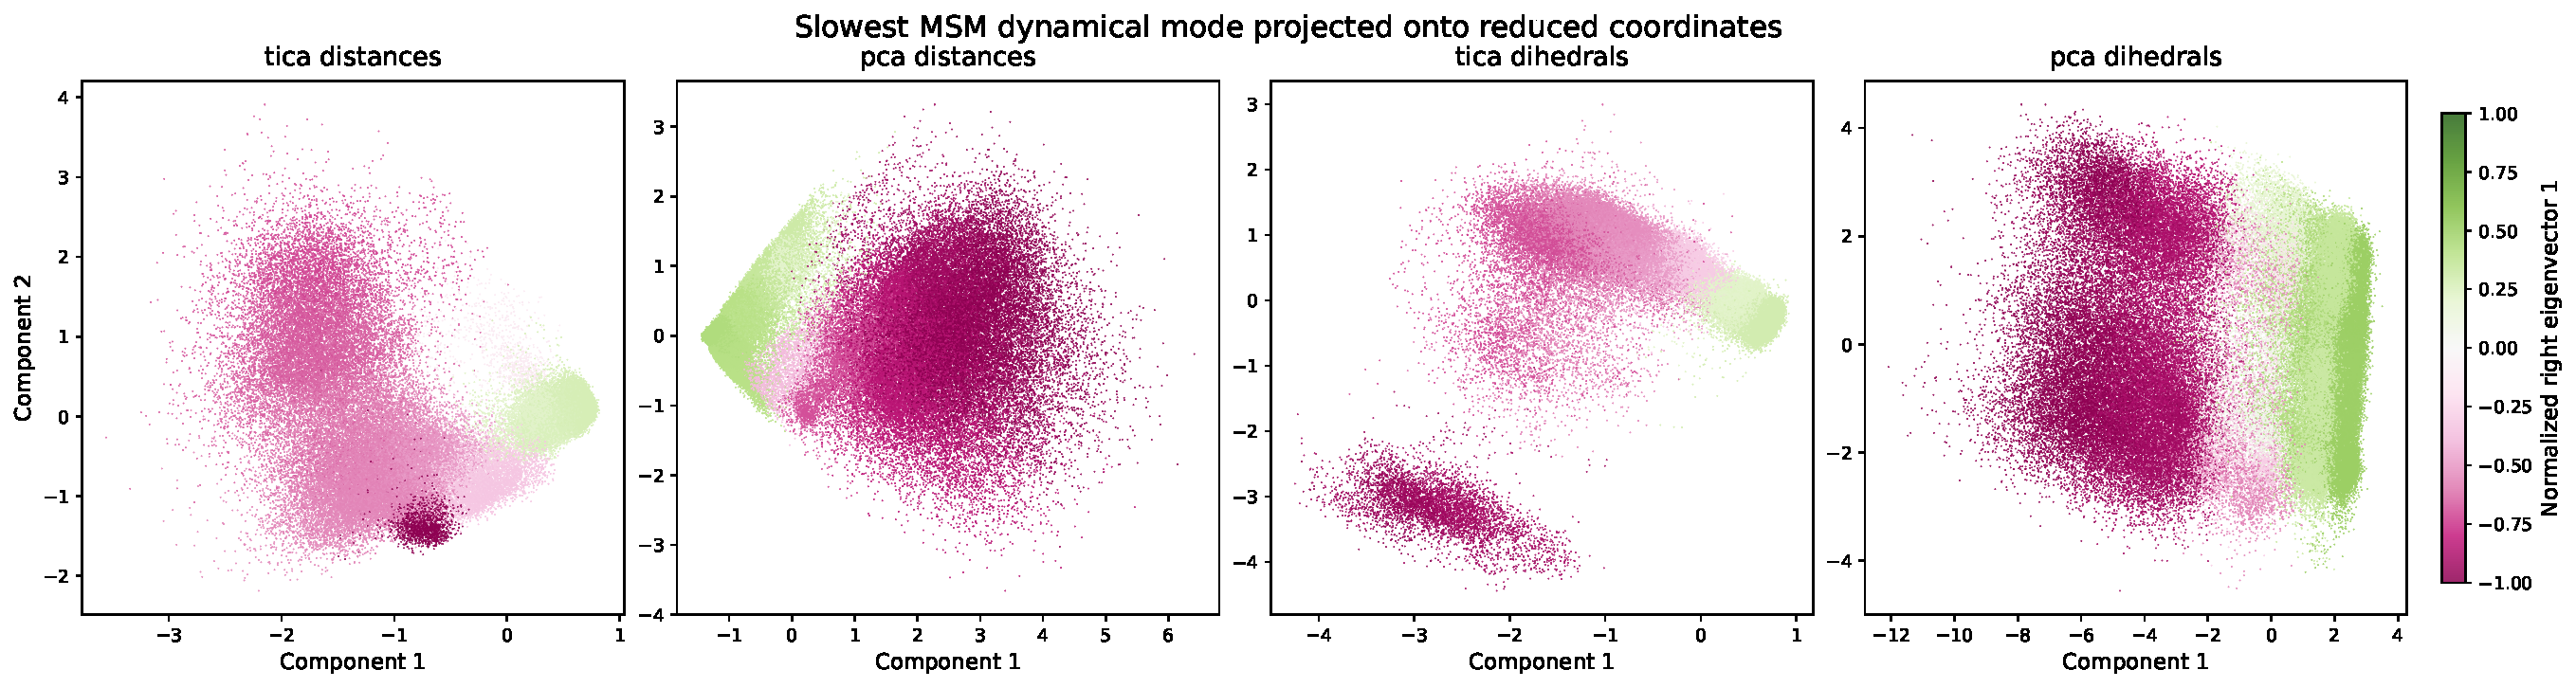
\includegraphics[width=0.8\linewidth]{figures/msm_right_eigenvector_1_projection.pdf}
    \vspace{1em}
    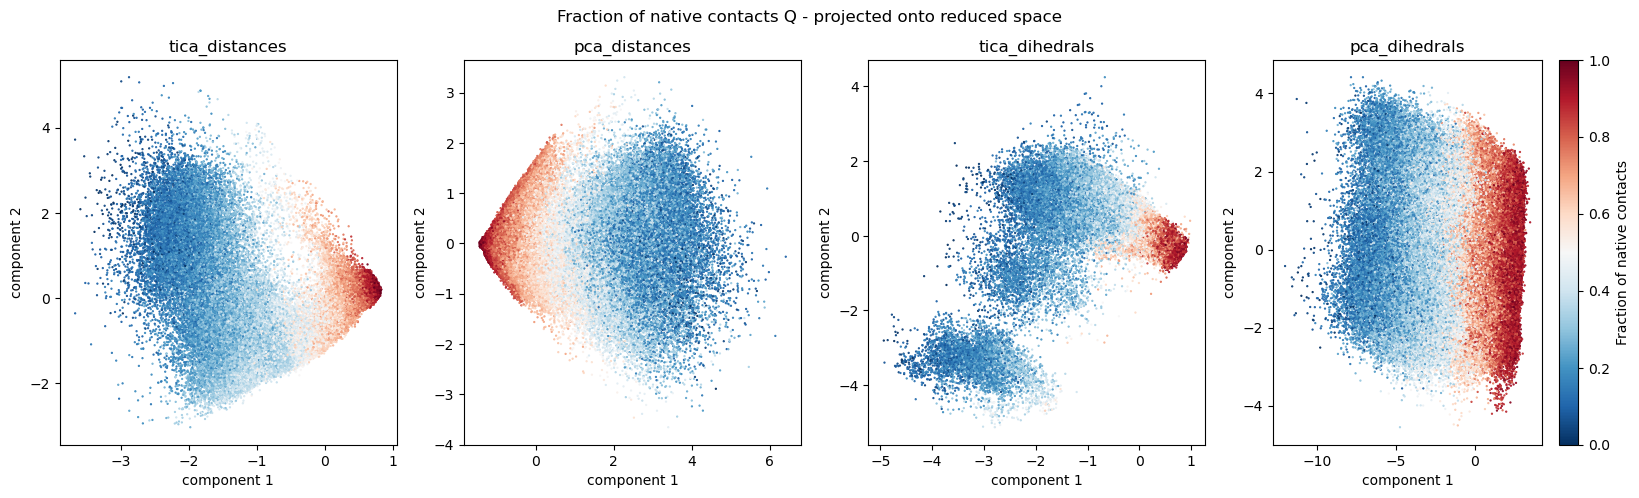
\includegraphics[width=0.8\linewidth]{figures/Q_reduced_projection.png}
    \caption{\footnotesize \textbf{Comparison between the slowest MSM relaxation mode and a structural folding descriptor.} 
    Top row: values of the first non-trivial eigenvector projected onto the first two components of the reduced coordinate space.
    Positive and negative components identify regions that exchange probability on the slowest resolved timescale of the Markov model. 
    Bottom row: projection of the fraction of native contacts, Q, onto the same coordinates. 
    The close correspondence between the eigenvector sign pattern and the distribution of $Q$ indicates that the slowest kinetic process 
    captured by the MSM is associated with the folding-unfolding transition.}
    \label{fig:eigenvectors}
\end{figure}



\begin{figure}[h!]
    \centering
    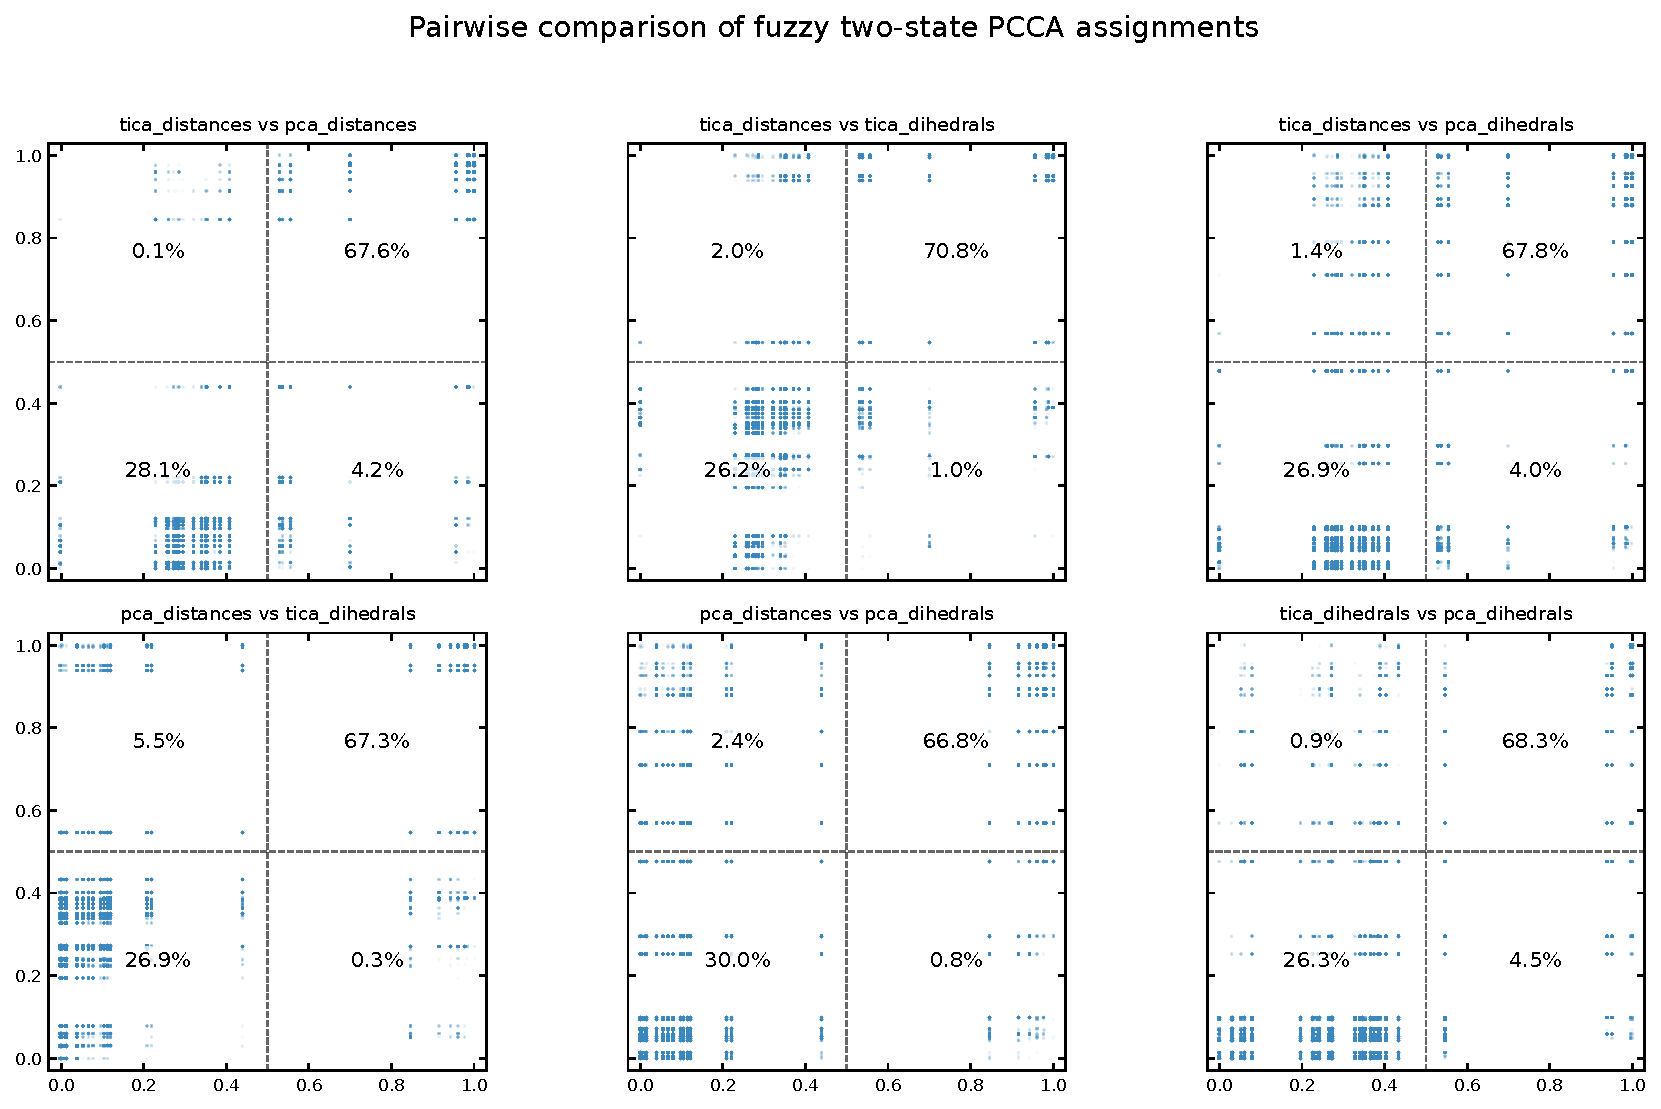
\includegraphics[width=0.8\linewidth]{figures/pairwise_pcca_membership_scatter_quadrants_report.pdf}
    \caption{\small \textbf{Fuzzy membership probabilities of the trajectory frames to the two macrostates across models.} Each panel shows the fuzzy membership probability of each frame in the trajectory to macrostate $0$ (denatured basin) and macrostate $1$ (native basin) for a different model. The models based on distances (tica-distances and pca-distances) show very similar distributions, while the tica-dihedrals model exhibits a broader distribution, particularly for frames assigned to the denatured basin. This indicates that the tica-dihedrals model has more uncertainty in assigning frames to the denatured basin.}
    \label{suppfig:fuzzy_memberships_models}
\end{figure}

\begin{table}[h!]
\caption{Pairwise correlations between frame-wise PCCA membership probabilities for the folded basin. Pearson correlations quantify linear agreement, whereas Spearman correlations quantify agreement in the rank ordering of frames along the folded-basin membership coordinate.}
\label{supptab:two_state_model_correlation}
\begin{tabular}{lcc}
\hline
Model pair & Pearson & Spearman \\
\hline
tICA distances -- PCA distances & 0.990 & 0.911 \\
tICA distances -- tICA dihedrals & 0.923 & 0.826 \\
tICA distances -- PCA dihedrals & 0.876 & 0.831 \\
PCA distances -- tICA dihedrals & 0.910 & 0.821 \\
PCA distances -- PCA dihedrals & 0.876 & 0.847 \\
tICA dihedrals -- PCA dihedrals & 0.885 & 0.930 \\
\hline
\end{tabular}
\end{table}


\begin{figure}[h!]
    \centering
    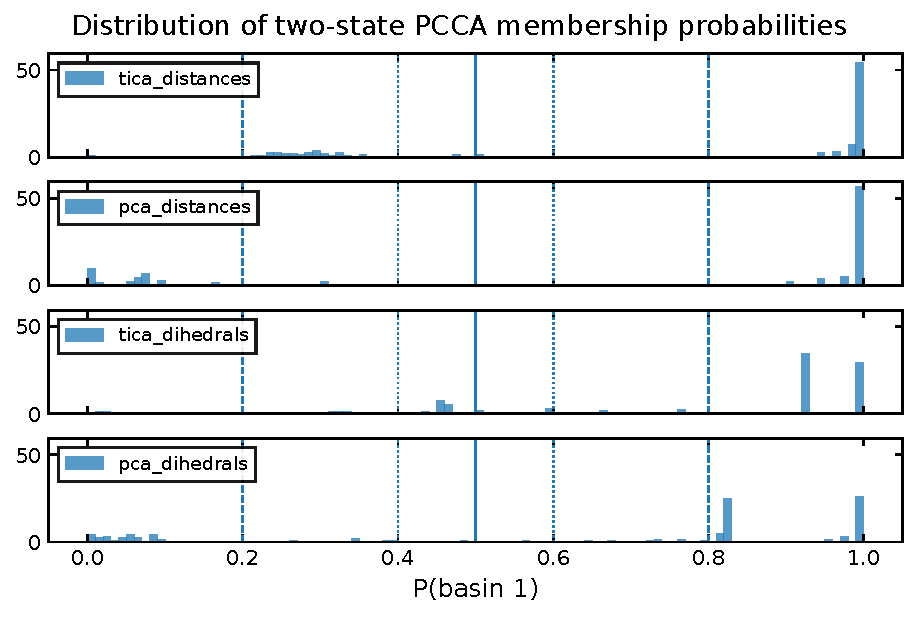
\includegraphics[width=0.4\linewidth]{figures/pcca_membership_probability_distributions.pdf}
    \caption{\small the distributions of fuzzy membership probabilities assigned to frames, for basin $1$ across the four models. }
    \label{suppfig:pcca_frames_prob_density}
\end{figure}

% ------------- Second eigenvector of tica models only -------------------------
\begin{figure}[!t]
    \centering
    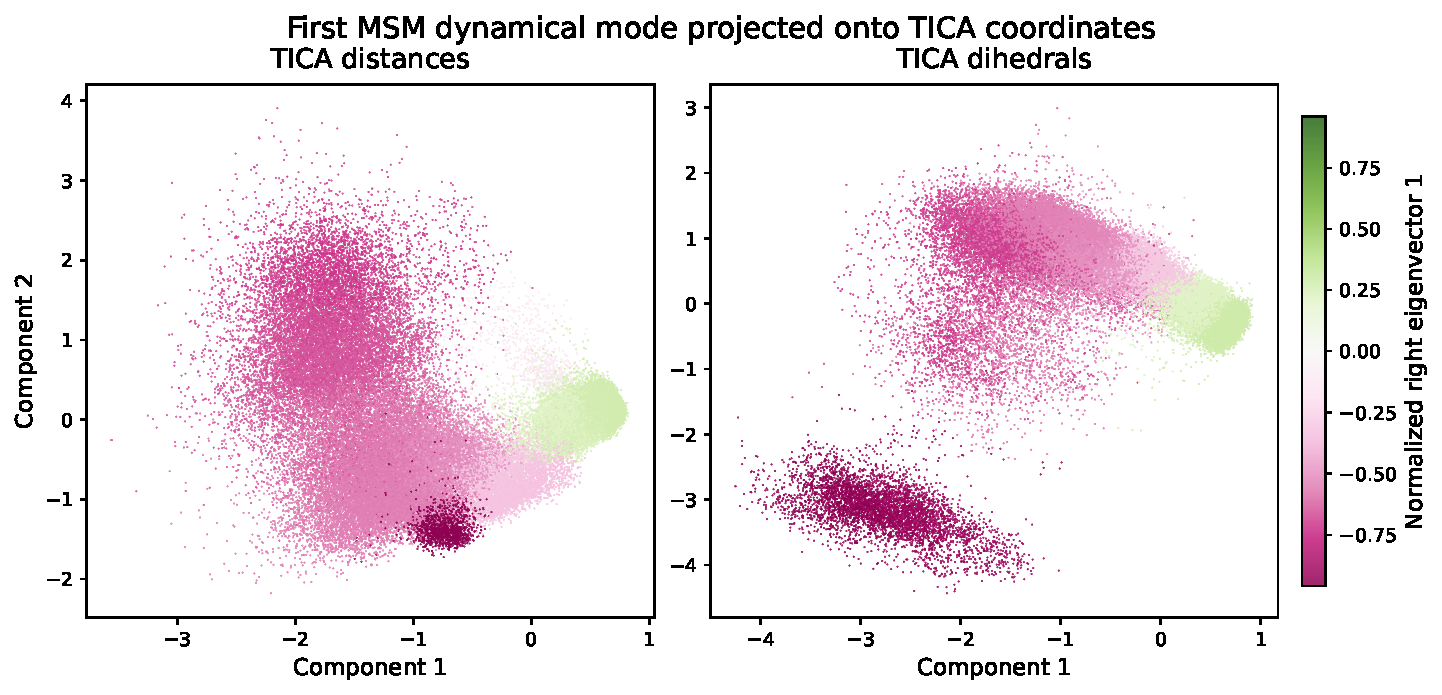
\includegraphics[width=0.45\linewidth]{figures/tica_right_eigenvector_1_projection.pdf}
    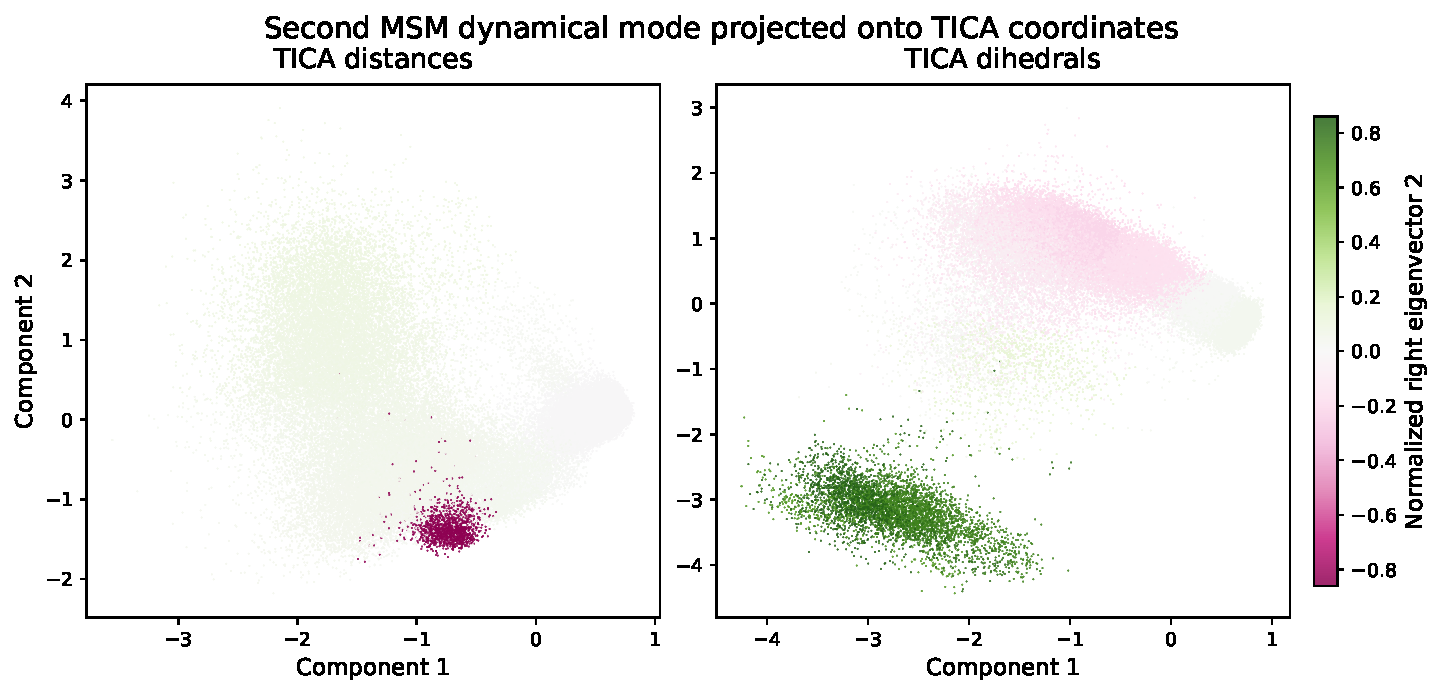
\includegraphics[width=0.45\linewidth]{figures/tica_right_eigenvector_2_projection.pdf}
    \vspace{1em}
    \caption{\footnotesize {First two non-trivial eigenvectors of the tICA-based MSMs projected onto the first two tICA coordinates.}}
    \label{fig:tica_second_eigvec}
\end{figure}






\section{Supplementary Methods}
\label{sec:SI_methods}
Here I provide the technical details of the procedure summarized in Methods.

\renewcommand{\thesubsection}{S\arabic{subsection}}
\setcounter{subsection}{0}

\subsection{Derivation of PCA and tICA}


\label{subsec:SI_dimred}
The presentation of tICA in this section follows closely that of \cite{my_tica_ref}.


PCA and tICA are both linear dimensionality reduction techniques, i.e. they project the data onto a linear subspace of the original feature space. 
Let $\{\mathbf{x}(t)\}_{t=0}^{T-1}$ be a multidimensional, discrete time-series, where each snapshot is a column vector, 
of dimension $D$, corresponding to an arbitrary, vectorized representation of a protein conformation (e.g. a set of dihedral angles). 
Suppose the data has been sampled from a \textit{stationary} and \textit{time-reversible} stochastic process. 
Without loss of generality, I assume that the data have been centered, $\mathbb E[\mathbf{x}] = 0 $. Using the braket notation $\bra{x} := \mathbf{x}^T, \ket{x} := \mathbf{x} $, I define the covariance matrix:


\begin{equation}
\mathbf{C}_0 := \mathbb{E}\!\left[\ket{x}\bra{x}\right]
\end{equation}

and the time-lagged covariance matrix:
\begin{align}
    \mathbf{C}_{0,\tau}:&= \mathbb{E}\left[\ket{x(t)}\bra{x(t + \tau)}\right].
\end{align}

For a stationary reversible process,
\begin{equation*}
\mathbf C_{0,\tau} = \mathbf C_{\tau,0}^{T} = \mathbf C_{\tau,0},
\end{equation*}
so that the lagged covariance matrix may be denoted simply by \(\mathbf C_\tau\).

If $\ket{\hat{u}}\bra{\hat{u}}$ is a projection operator (i.e. $\ket{\hat{u}}$ is a unit vector), then:

\begin{equation}
    \bra{\hat{u}}\mathbf{C}_0\ket{\hat{u}} = \mathbb{E}[\braket{\hat{u}|x}\braket{x|\hat{u}}] = \mathbb{E}[\braket{\hat{u}|x}^2]
\end{equation}
is the variance of the projection of the data along $\ket{\hat{u}}$, and

\begin{align}
    \label{eq:autocorrelation}
    \textrm{ACF}_{\hat{u}}(\tau) &=\frac{\bra{\hat{u}}\mathbf{C}_{\tau}\ket{\hat{u}}}{\bra{\hat{u}}\mathbf{C}_{0}\ket{\hat{u}}} \notag \\
    \\ &= \frac{\mathbb{E}[\braket{\hat{u}|x(t)}\braket{\hat{u}|x(t+\tau)}]}{\mathbb{E}[\braket{\hat{u}|x}^2]} \notag 
\end{align}

its autocorrelation at lag time $\tau$.

\vspace{0.5em}

\noindent \textbf{PCA} seeks the direction of maximal variance. The first principal component is defined as
\begin{align}
\ket{\hat{u}_1} =& \arg\max \bra{\hat{u}}\mathbf{C}_0\ket{\hat{u}}  \notag \\
&\text{subject to}\,\,\|\hat{u}\|=1
\end{align}

this optimization problem can be solved introducing a Lagrange multiplier $\lambda$, and the stationarity condition yields

\begin{equation}
\mathbf{C}_0 \ket{\hat{u}_i} =\lambda_i \ket{\hat{u}_i},
\end{equation}

i.e. the projection versor is an eigenvector of the covariance matrix. The corresponding eigenvalue equals the variance of the data projected onto the principal component:

\begin{equation*}
\bra{\hat{u}_i}\mathbf{C}_0\ket{\hat{u}_i} = \lambda_i \cdot \braket{\hat{u}_i|\hat{u}_i} = \lambda_i.
\end{equation*}

Then the second principal component is defined as the direction of maximal variance orthogonal to the first, giving the 
optimization problem:
\begin{align}
\ket{\hat{u}_2} = &\text{argmax}\bra{u}\mathbf{C}_0\ket{u} \notag \\
&\text{subject to}  \,\, \braket{u|u} = 1 \notag \\
&\text{and}   \,\, \braket{u|\hat{u}_1} = 0
\end{align}

which again can be solved with Lagrange multipliers. Iterating, this implies that the principal components form an orthonormal basis of eigenvectors of the covariance matrix, i.e. they diagonalize the covariance matrix.
Dimensionality reduction ($d < D$) is achieved by taking the components along the first $d$ 
principal components $\{\ket{\hat{u}_1}, \ldots, \ket{\hat{u}_d}\}$.


\begin{equation}
z_i = \braket{\hat{u}_i|x}, \qquad \mathbf z = U^T \mathbf x.
\end{equation}

This is a linear projection onto an ortonormal basis:

\begin{equation*}
    \ket{x} \rightarrow \ket{z} := \sum_{i = 1}^{d}\, \braket{x | \hat{u}_i}\, \ket{\hat{u}_i} 
\end{equation*}

By construction, in the reduced space components are uncorrelated and ordered by decreasing variance:

\begin{equation}
 \mathbb{E}\!\left[\ket{z}\bra{z}\right] = \text{diag}(\lambda_1,\, \cdots \lambda_d)
\end{equation}
\vspace{1em}

\noindent \textbf{tICA} Unlike PCA, tICA \cite{my_tica_ref} seeks directions $\ket{u}$ that maximize the autocorrelation Eq.\eqref{eq:autocorrelation} at a fixed lag time $\tau$. The lagtime $\tau$ is a free parameter.
The autocorrelation is invariant under scaling of the projection vector $\ket{u}$. Differently from PCA, the normalization constraint is usually implemented as $\bra{u}\mathbf{C}_{0}\ket{u}=1$, as this choice simplifies the optimization problem.
Formally, tICA solves the optimization problem:

\begin{align}
    \label{eq:generalized_eigenvalue_problem}
\ket{\hat{u}_1} =& \text{argmax}\bra{u}\mathbf{C}_{\tau}\ket{u} \notag \\
&\text{subject to}  \,\, \bra{u}\mathbf{C}_{0}\ket{u} = 1
\end{align}

using the same procedure as for PCA, I can solve this with Lagrange multipliers, and show that


\begin{equation}
\mathbf{C}_{\tau}\ket{\hat{u}_1}
=
\lambda_1
\mathbf{C}_{0}\ket{\hat{u}_1},
\end{equation}.

The generalized eigenvalue $\lambda_i$ is equal to the autocorrelation of the projected coordinate $\braket{\hat{u}_i|x(t)}$ at lag time $\tau$. Assuming that this coordinate approximates a single relaxation mode of the dynamics, its autocorrelation decays exponentially, yielding

\begin{equation}
    \label{eq:eigvals_and_timescales}
    \lambda_i \approx e^{-\tau/t_i},
\end{equation}

where $t_i$ is the corresponding relaxation timescale. In practice, the relation is approximate because a tIC may contain contributions from multiple dynamical modes.

Similarly as done with PCA, I can iterate this procedure and define the second tIC as the direction of maximal autocorrelation at lag time $\tau$ that is \textit{uncorrelated} with the first:


\begin{align}
\ket{\hat{u}_2} = &\text{argmax} \bra{u}\mathbf{C}_{\tau}\ket{u} \notag \\
&\text{subject to}  \,\, \bra{u}\mathbf{C}_{0}\ket{u} = 1 \notag \\
&\text{and}   \,\, \bra{u}\mathbf{C}_{0}\ket{\hat{u}_1} = 0
\end{align}

the solution $\ket{\hat{u}_1}$ is again a solution of the same generalized eigenvalue problem as in Eq.\eqref{eq:generalized_eigenvalue_problem}.
generalized eigenvalue problem.
Dimensionality reduction ($d < D$) is achieved by taking the components of the data $\mathbf{x}(t)$ along the first $d$ tICs $\{\ket{\hat{u}_1}, \ldots, \ket{\hat{u}_d}\}$.

\begin{equation}
    \mathbf{z}(t) = (\braket{x(t) | \hat{u}_i}, \cdots, \braket{x(t) | \hat{u}_d})
\end{equation}

By construction, in the reduced space components $z_i$ have unit variance, are uncorrelated at zero lag,  and are ordered by decreasing autocorrelation at lag time $\tau$.

\begin{equation}
    \label{eq:original_tica}
 \mathbb{E}\!\left[\ket{z}\bra{z}\right] = \mathbb{I}
\end{equation}

\vspace{1em}


\noindent \textbf{tICA as a diagonalization in the whitened coordinate space}
It is worth noting that unlike in PCA, the tIC vectors are generally not orthogonal under the standard Euclidean inner product. Instead, as I said, they satisfy the generalized orthogonality relation
$$
\bra{u_i}\mathbf C_0\ket{u_j}=\delta_{ij}.
$$
i.e. they corresponding components $z_i$ and $z_j$ are \textit{uncorrelated} at zero lag. Nevertheless, the tICA procedure can be reformulated as a standard eigenvalue problem in a transformed coordinate system. The key idea is to first apply a whitening transformation, which rescales and rotates the original data so that all directions have unit variance and are mutually uncorrelated. Define the ZCA whitening transformation

\begin{equation*}
\ket{y} = \mathbf C_0^{-1/2} \ket{x}
\end{equation*}

where $C_0^{-1/2}$ is symmetric and positive definite. By construction, the covariance matrix in the transformed space is the identity:

\begin{equation*}
\mathbb E\left[\ket{y}\bra{y}\right] = \mathbf{C}_0^{-1/2} \mathbf{C}_0 \mathbf{C}_0^{-1/2} = \mathbf I.
\end{equation*}

and time-lagged covariance matrix in the whitened space is

\begin{equation*}
\hat{\mathbf{C}}_\tau = \mathbf C_0^{-1/2} \mathbf C_\tau \mathbf C_0^{-1/2}
\end{equation*}

$\hat{\mathbf{C}}_\tau$ is symmetric and can thus be diagonalized:,

\begin{equation*}
\hat{\mathbf{C}}_\tau \ket{v_i} = \lambda_i \ket{v_i}, \qquad
\braket{v_i|v_j} = \delta_{ij}.
\end{equation*}

If $\ket{u_i}$ solves the tICA problem \eqref{eq:generalized_eigenvalue_problem}, then $\ket{v_i} = \mathbf C_0^{1/2} \ket{u_i}$ is an eigenvector of $\hat{\mathbf{C}}_\tau$ with the same eigenvalue.

Indeed, multiplying the generalized eigenvalue problem \eqref{eq:generalized_eigenvalue_problem} from the left by $\mathbf C_0^{-1/2}$ and defining
$\ket{v_i} = \mathbf C_0^{1/2}\ket{u_i}$ yields

\begin{equation*}
\hat{\mathbf C}_\tau \ket{v_i} = \lambda_i \ket{v_i}.
\end{equation*}

Consequently, the tICA components $z_i$ correspond to the ortogonal projection of the whitened data $\mathbf{y}$ onto the ortonormal basis defined by $\{\ket{v_i}\}$:

\begin{equation*}
z_i(t) = \braket{x(t)|u_i} = \braket{x(t) | C_0^{-1/2} v_i}  = \braket{y(t) | v_i}.
\end{equation*}


\vspace{1em}
\noindent \textbf{Alternative generalized eigenvector normalizations for tICA}\newline 
The construction presented above corresponds to the original formulation of tICA, in which the covariance matrix of the transformed data is the identity \eqref{eq:original_tica}.
HoIver, alternative rescaling of the transformed coordinates have been used in the literature and are usually implemented in softwares to endow Euclidean distances in the reduced space with a more direct kinetic interpretation. These can 
be particularly useful when the tICA coordinates are subsequently clustered to construct a Markov state model, as I do in this work.

The most commonly used choice is the \textit{kinetic map} in which each tIC component $z_i$ is multiplied by its corresponding eigenvalue,

\begin{equation}
\tilde z_i(t) = \lambda_i z_i(t).
\end{equation}

With this normalization, the coordinates representing the sloIst processes "Iight more", and a unit step in those directions in the reduced space is assigned a larger distance.
An alternative is the \textit{commute map}, where each coordinate is rescaled according to its implied timescale,
\begin{equation}
\tilde z_i(t) = \sqrt{\frac{t_i}{2}} z_i(t), \qquad t_i = -\frac{\tau}{\ln \lambda_i}.
\end{equation}
With this normalization, Euclidean distances approximate commute distances, i.e. the expected time required to travel from one configuration to another and back. This is a variation on the same idea behind the kinetic map, being eigenvalues and timescales connected by \eqref{eq:eigvals_and_timescales}.



\subsection{Elements of Markov theory}
\label{suppsec:markov_theory}

\textcolor{gray}{
Markovianity assessment and optimal lagtime choice was performed through the implied-timescale convergence test. The i-th implied timescale estimated at lag $\tau$,  $t_i(\tau)$ is given by the relation:
\begin{equation}
t_i(\tau) = -\frac{\tau}{\ln \lambda_i(\tau)}
\end{equation}
where $\lambda_i(\tau)$ is the $i$-th eigenvalue ($i \geq 2$) of the transition matrix estimated at lag time $\tau$.
It is known that the true timescales of the underlying continuous-state Markov process, $t_i^{*}$, are approximated from below ($t_i(\tau) \leq t_i^{*}$) and the relative error decreases as
i) the discretization error decreases or ii) the lagtime $\tau$ increases. With this consideration, the implied timescale test consists in plotting $t_i(\tau)$ as a function of $\tau$ and looking for a region of approximate convergence, where the estimated timescales are approximately constant.
The lagtime is selected as the minimum value in the region of convergence, as this choice minimizes the loss of temporal resolution while ensuring that the process of interest is approximately Markovian \cite[Ch. 4.7]{thebible}. 
}

\textcolor{gray}{
After selecting the MSM lag time based on the implied timescale convergence analysis, model quality was further assessed using an autocorrelation function test. 
While a direct Chapman-Kolmogorov (CK) test provides a stringent validation of Markovianity, its application at the microstate level becomes impractical for models containing hundreds of states, 
as it requires comparing $T(k\tau)$ and $[T(\tau)]^k$ entry-wise, and summary statistics are needed which could be difficult to interpret. 
Instead, following the approach suggested by [Chap. 2.4.2]\cite{thebible}, model predictions were evaluated through the autocorrelation function of a physically meaningful observable.
As an observable, the root-mean-square deviation (RMSD) from the crystal structure was chosen. For each microstate, a representative observable value was obtained by averaging the RMSD over all trajectory
frames assigned to that microstate. The MSM prediction for the autocorrelation function was then computed from the spectral decomposition of the transition matrix,
}

\noindent The dynamics encoded by a Markov state model can be understood through the eigendecomposition of its transition matrix $\mathbf{T}$.
For consistency with the notation used in the Python package deeptime, let us consider the transition matrix $\mathbf{T}$ as a row-stochastic matrix, i.e. $T_{ij}$ is the probability of transitioning from state $i$ to state $j$ in one lag step:
\begin{equation*}
    \sum_j T_{ij} = 1, \qquad T_{ij} \geq 0.
\end{equation*}
Probability distributions are represented as row vectors, and evolve as:
\begin{equation*}
\mathbf{p}(n) = \mathbf{p}(0)\mathbf{T}^n,
\end{equation*}
where $\mathbf{p}(0)$ is the initial distribution and $\mathbf{p}(n)$ is the distribution after $n$ lag steps.
The transition matrix admits a spectral decomposition of the kind:
\begin{equation*}
\mathbf{T} = \sum_i \lambda_i \mathbf{r}_i \mathbf{l}_i^{\mathrm T},
\end{equation*}
where $\lambda_i$ are the eigenvalues, and $\mathbf{r}_i$ and $\mathbf{l}_i$ are the corresponding right and left eigenvectors, satisfying:
\begin{equation*}
\mathbf{T}\mathbf{r}_i=\lambda_i\mathbf{r}_i,
\qquad
\mathbf{l}_i^{\mathrm T}\mathbf{T}=\lambda_i\mathbf{l}_i^{\mathrm T}.
\end{equation*}


The probability distribution after $n$ lag times can therefore be written as

\begin{equation*}
\mathbf{p}(n)=
\mathbf{p}(0)\mathbf{T}^{,n}=
\sum_i
c_i\, \cdot \lambda_i^n \cdot \mathbf{l}_i,
\end{equation*}

where the coefficients $c_i = \mathbf{p}(0)\mathbf{r}_i$ depend on the initial condition. The dominant eigenvalue is $\lambda_1=1$ and corresponds to the equilibrium distribution. All other modes decay exponentially with characteristic relaxation times

\begin{equation*}
t_i
-\frac{\tau}{\ln \lambda_i},
\end{equation*}

where $\tau$ is the MSM lag time.

The left eigenvectors therefore describe the spatial structure of the relaxation processes occurring on the corresponding timescales. States with eigenvector components of opposite sign exchange probability during the relaxation process, while the magnitude of each component quantifies the degree to which that state participates in the process. The instantaneous probability flux associated with a mode can be visualized from the change in the probability distribution after one lag step,

\begin{equation*}
\Delta\mathbf{p} = 
\mathbf{p}\mathbf{T} - \mathbf{p} = {\color{orange} TODO: complete}
\end{equation*}

For reversible Markov models obeying detailed balance, left and right eigenvectors contain equivalent information and are related through the equilibrium population matrix $\boldsymbol{\Pi}$,

\begin{equation*}
\mathbf{l}_i
\boldsymbol{\Pi},\mathbf{r}_i .
\end{equation*}

Consequently, the right eigenvectors may be interpreted as equilibrium-population-weighted versions of the relaxation modes.



Autocorrelation of an observable $\theta$ can be expressed in terms of the spectral decomposition of the transition matrix. Let $\theta_i$ be the value of the observable in microstate $i$, and let $\langle \theta, \mathbf{r}_i\rangle_\pi$ denote the inner product weighted by the stationary distribution $\pi$. The autocorrelation function at lag time $n$ is then given by

\begin{align}
c(n)
&=
\frac{
\sum_{i=1}^{N}
\lambda_i^{n}\,
\langle \theta,\mathbf{r}_i\rangle_\pi\,
\langle \theta,\mathbf{l}_i\rangle
}
{
\sum_{i=1}^{N}
\langle \theta,\mathbf{r}_i\rangle_\pi\,
\langle \theta,\mathbf{l}_i\rangle
}
\notag \\
&\equiv
\frac{
\sum_{i=1}^{N}
\lambda_i^{n}\,
\langle \theta,\mathbf{l}_i\rangle^2
}
{\sum_{i=1}^{N}\, \langle \theta,\mathbf{l}_i\rangle^2} \notag
\end{align}

where $\lambda_i$ and $(\mathbf{l}_i, \mathbf{r}_i)$ denote the eigenvalues and (left, right) eigenvectors of the transition matrix (in row-stochastic notation), $\pi$ the stationary distribution,
and ($\boldsymbol{\theta}$) is the vector of microstate-averaged RMSD values. Equivalence between the two reported formula hold because of the detailed balance assumption.
%


\textcolor{gray}{
The dynamical processes captured by each MSM were characterized through the spectral decomposition of the transition matrix (see Supplementary Information \ref{si:spectral} for details). 
The eigenvalues were converted into relaxation timescales, while the corresponding eigenvectors were used to identify the states participating in each relaxation process. 
States with eigenvector components of opposite sign exchange probability on the associated timescale, whereas the magnitude of each component reflects the degree of participation
of that state in the process. For reversible models satisfying detailed balance, left and right eigenvectors contain equivalent kinetic information
and are related through the equilibrium distribution.
The signs of eigenvectors components provide a criterion for defining partitions in the microstate model. This is systematically done through the algorithm PCCA++ \cite[Ch. 2.5.1 and 2.5.2]{thebible}. I use this method to connect
the slowest exchange modes in the markov chain to the thermodynamics of the protein, although the two are not strictly the same thing. 
}
\vspace{0.1em} \newline \textit{Lagtime choice:}
Estimation of the transition matrix requires specification of the lag time $\tau$ ($= 1, 2, 3\cdots$ in number of frames) at which to count transitions between states. Choice of lag time is done through the
timescale convergence test. Briefly (see Supplementary Methods \ref{suppsec:markov_theory} for more details), the transition matrix $T(\tau)$  is estimated at different lag times and its eigenvalues are used to compute the implied timescales $t_i(\tau)$, which are then plotted as a function of $\tau$. 
If the Markovian assumption is valid, the implied timescales should be approximately constant for sufficiently large $\tau$. The lag time is then selected as the minimum value in the region of convergence, as this choice minimizes the loss of temporal resolution while ensuring that the process of interest is approximately Markovian\cite[Ch. 4.7]{thebible}.
\vspace{0.1em} \newline \textit{MSM validation:} to validate the model against the original trajectory, I compare the autocorrelation function of the root mean square deviation (RMSD) to the crystal structure computed from the trajectory (\texttt{hp35.crystaldist}) and predicted by the MSMs (see \ref{suppsec:markov_theory}).
%

\end{document}